\documentclass[12pt]{article}
\usepackage[utf8]{inputenc}
\usepackage{polski}
\usepackage{hyperref}
\usepackage{listings}
\usepackage{mathtools}
\usepackage{graphicx}
\usepackage{fullpage}
\usepackage{float}
\usepackage{caption}
\usepackage{parskip}
\usepackage{subcaption}
\title{Teoria i Inżynieria Ruchu Teleinformatycznego \\ Sprawozdanie z projektu}
\author{Ewelina Kawecka (201420) \\ Michał Smyk (203254)}
\graphicspath{ {gfx/} }
\begin{document}
\maketitle
\thispagestyle{empty}
\clearpage
\setcounter{page}{1}

\section{Wstęp}
Celem całości projektu było stworzenie programu, który na podstawie historii ruchu w sieci komputerowej będzie w stanie przeanalizować ruchu pod kątem interesujących właściwości, które mogą być w tej historii zawarte. W ramach tego sprawozdania opisana jest część projektowa odpowiedzialna za ekstrakcję danych z plików PCAP, zawierających nagrane informacje na temat historii ruchu w sieci. 

\section{Opis problemu}
Głównym problemem, na którym skupia się ta część projektu jest ekstrakcja i filtrowanie danych zawartych w pliku PCAP. Z racji, że w plikach tych znajdują się również dodatkowe informacje, które ze względu na brak przydatności do celów zadania powinny zostać odfiltrowane. Pozostałe dane, które przechowują przydatne informacje powinny zostać przetworzone w taki sposób, aby umożliwić odczytanie z nich informacji, które interesują osobę wykorzystującą program. Filtracja i ekstrakcja danych podzielona została na kilka etapów, które w postaci funkcji udostępniane są przez program. Funkcje te przedstawia rysunek \ref{img:funkcje}.

\begin{figure}[h]
\centering
\caption{Atomowe funkcje opracowane w ramach tej części projektu}
\label{img:funkcje}
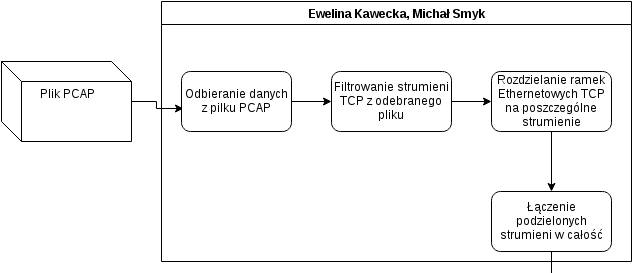
\includegraphics[width=0.7\textwidth]{Wykres.png}
\end{figure}


Zgodnie z zaleceniami prowadzącego każda atomowa funkcja realizowana przez program udostępniona jest w formie usługi - szczegółowe informacje na ich temat dostępne są w rozdziale \ref{dzialanie}. 


\section{Opis implementacji programu}
\label{dzialanie}
\section{Przykładowe wywołanie}
Program wywołujemy poprzez uruchomienie wszystkich usług, które składają się na jego elementy:
%\begin{itemize}
%\item main.py
%\item frame filter.py
%\item merger.py
%\item receiver.py
%\end{itemize}

%Dopiero po uruchomieniu tych plików, możemy za pomocą pliku \emph{sender.py} wysłać plik z rozszerzeniem %\emph{.pcap} jako pierwszy argument, aby wysłać zadany plik do poszczególnych usług w celu ich dalszego %przetworzenia. 
\end{document}
